\title{
    MS-E2112 - Multivariate Statistical Analysis\\
    Project Assignment\\
    ~\\
    \large{What factors are related to good performace in my chess games against stronger opponents}
}
\author{Tommi Summanen \\ tommi.summanen@aalto.fi}
\date{\today}

\documentclass[12pt]{article}
\usepackage{amsmath}
\usepackage{parskip}
\usepackage[sorting=none]{biblatex}
\usepackage[pdftex]{graphicx}
\usepackage{listings}

% for adding units in side math mode
\newcommand{\un}[1]{\ensuremath{\ \mathrm{#1}}}

\addbibresource{refs.bib}

\begin{document}

%\maketitle
%\newpage
%\tableofcontents

\begin{center}
    \Large{\bf MS-E2112 - Multivariate Statistical Analysis\\
    Project Assignment}\\
    \vspace{10pt}
    \large{What factors are related to good performace in my chess games against stronger opponents}
\end{center}
\vspace{10pt}
\begin{center}
    Tommi Summanen\\ 
    {\textit{{\small{
    Aalto University School of Science, Department of Mathematics and Systems Analysis\\
    tommi.summanen@aalto.fi}}}}
\end{center}

% Maximum points are 6 and the 6 points are divided as follows.

% Intro (description of the research question and of the data source or data collection) --- max 0.5 p.
\section{Introduction}

In this report I analyze what factors are related to good performance i.e. high winning probability in chess games against stronger opponents. My data set consists of chess games that author of this report has played between 2016-2021 on website lichess.org under username aitotumainen against other human players around the world.

In section \ref{sec:univariate} I introduce variables in the data and build understanding of the data through visualizations. In section \ref{sec:bivariate} I perform bivariate correspondence analysis on the data. In section \ref{sec:multivariate} I use multiple correspondence analysis to gain more insight about performance in chess games. Finally in section \ref{sec:conclusions} I summarize results, discuss about their limitations and propose ideas for further research.

% Univariate analysis (description of the variables, summary statistics, visualization) --- max 1p.
\section{Univariate analysis}
\label{sec:univariate}

\subsection{Raw data}

In my data one chess game forms one data point. Lichess API allows me to extract following information regarding one game: string describing the event (for example whether it was casual or rated game i.e. affected players rating \cite{elo} or no), URL to the game, date and time when game occurred, usernames of both players, ELO rating of both players, result of the game, rating change of both players after the game, game variant and time control, reason for game result which in addition winning by mate can be a problem with internet connection, ECO code \cite{eco} of the opening and all moves in the game using algebraic notation \cite{notation}. In addition to these possible titles of the player such as International Master or Grand Master are given and well as two additional fields regarding Chess 960 variant games. Following provides an example of the API output:

\begin{lstlisting}[breaklines]
    [Event "Rated Rapid game"]
    [Site "https://lichess.org/oykful3u"]
    [Date "2020.06.19"]
    [White "martoj13"]
    [Black "aitotumainen"]
    [Result "1-0"]
    [UTCDate "2020.06.19"]
    [UTCTime "06:12:07"]
    [WhiteElo "1920"]
    [BlackElo "1919"]
    [WhiteRatingDiff "+6"]
    [BlackRatingDiff "-6"]
    [Variant "Standard"]
    [TimeControl "600+0"]
    [ECO "B01"]
    [Termination "Normal"]
    1. e4 d5 2. e5 Nc6 3. Bb5 a6 4. Bxc6+ bxc6 5. d4 Bf5 6. Nd2 e6 7. c3 c5 8. Ne2 cxd4 9. Qa4+ Qd7 10. Qxd7+ Kxd7 11. cxd4 Bd3 12. Nf4 Bb5 13. a3 c5 14. dxc5 Bxc5 15. Nb3 Bf8 16. Nd4 Ne7 17. Be3 Nf5 18. Nxf5 exf5 19. Nxd5 Re8 20. f4 Bc6 21. Rd1 Bxd5 22. Rxd5+ Kc6 23. Rd2 f6 24. Bd4 g5 25. g3 h5 26. Kf2 h4 27. Rc1+ Kb7 28. Rcc2 hxg3+ 29. hxg3 Rh2+ 30. Kg1 Rh3 31. Kg2 Rh7 32. exf6 gxf4 33. gxf4 Bh6 34. Rf2 Re4 35. Be5 Bf8 36. Rf3 Kb6 37. Rg3 Bc5 38. Rg7 Rh4 39. f7 Re1 40. Rxc5 1-0
\end{lstlisting}

In following analysis I study only relations between Result, UTCDate, UTCTime, WhiteElo, BlackElo, Variant and TimeControl. By common sense text strings such as username and event description shouldn't affect the game result. Rating differences are calculated after the game has ended so they can't be explaining factors for the result of the game. I also discard game opening and move information. While this information is definitely meaningful analyzing it would be very complex as already after two moves standard chess game can be in 400 different states and tree of possible game continuations grows unmanageable. For those who are interested on how opening affects game's outcome Lichess Opening Explorer \cite{opening_explorer} and Lichess Game Insights \cite{insights} offer tools for such analysis.

\subsection{Summary statistics from my games}

In total I have played 9085 chess games between 15.02.2016 - 25.03.2021 on this site. Table \ref{tbl:results by variant} shows how games are distributed between different variants \cite{variants} and how game results are distributed inside variant. I have made distinction inside standard chess between games with at least 10 minutes and games with less than 10 minutes on the clock as amount of available time changes nature of the game significantly. In proceeding analysis I will only focus on standard and crazyhouse variants as they have the greatest number of games.

\begin{table}[ht]
    \centering
    \label{tbl:results by variant}
    \caption{Results by chess variant.}
    \begin{tabular}{lllll}
    Chess variant    & wins & draws & losses & win rate\\
    \hline
    Atomic& 138& 7& 120& 0.52 \\
    Crazyhouse& 1732& 15& 2535& 0.40 \\
    Standard short time control& 1162& 70& 1581& 0.41 \\
    From Position& 5& 0& 5& 0.5 \\
    Standard long time control& 794& 79& 712& 0.50 \\
    King of the Hill& 34& 0& 33& 0.51 \\
    Chess960& 9& 1& 12& 0.41 \\
    Three-check& 6& 0& 9& 0.4 \\
    Racing Kings& 8& 0& 8& 0.5 \\
    Horde& 1& 0& 7& 0.13 \\
    Antichess& 2& 0& 0& 1.0
    \end{tabular}
\end{table}


\subsection{Exploratory visualizations of the game data}

Figure \ref{fig:games vs time of day} shows who many games I have played at each hour of day and how many of them I have won and lost and their difference. Image shows that on short standard games and crazyhouse games I am losing more often than winning and on the other hand playing long standard games I win more often. This is consistent with figures in table \ref{tbl:results by variant}. One interesting observation is that between 2 and 3 PM I seem to perform unusually well when playing long standard chess as I win two thirds of my matches. Similarly I win half my crazyhouse games while on other hours of day I am losing more often. Only reason I think of causing this is my habit to drink cup of coffee around that time of day which probably gives me a cognitive boost. 


\begin{figure}[ht!]
    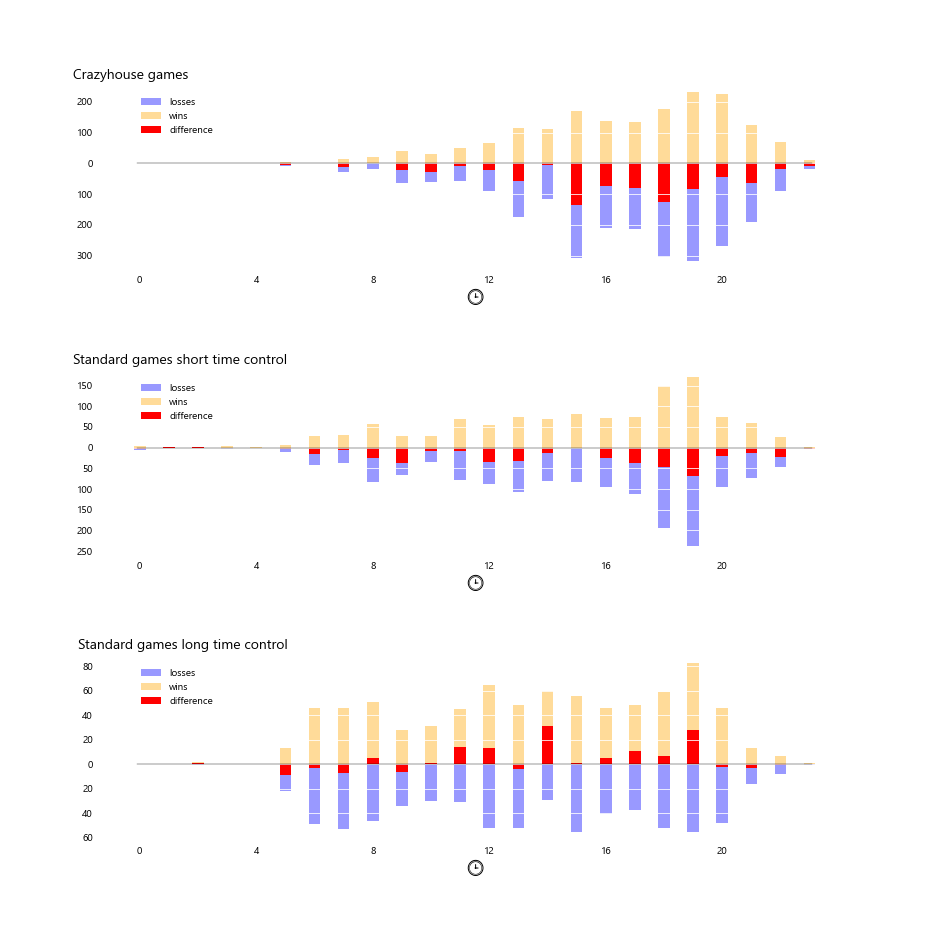
\includegraphics[width=\textwidth]{../img/games_vs_time_of_day.png}
    \caption{Wins and losses with respect to the time of the day.}
    \label{fig:games vs time of day}
\end{figure}

Figure \ref{fig:winning probabilities} shows histogram where rating difference of me and my opponent is divided to 20 equally wide bins and winning probability inside each bin is calculated. In standard chess (both long and short) winning probability seems to decrease in remarkably linear fashion with respect to increasing opponent strength. On the other hand crazyhouse variant has long tails: I have won opponents that are over 800 rating points better than me and vice versa also lost to opponent that are much weaker than me. It must be noted in this image middle bins contain much more data than bins on edges and also selected number of bins affects to the appearance of the graph.

\begin{figure}[ht!]
    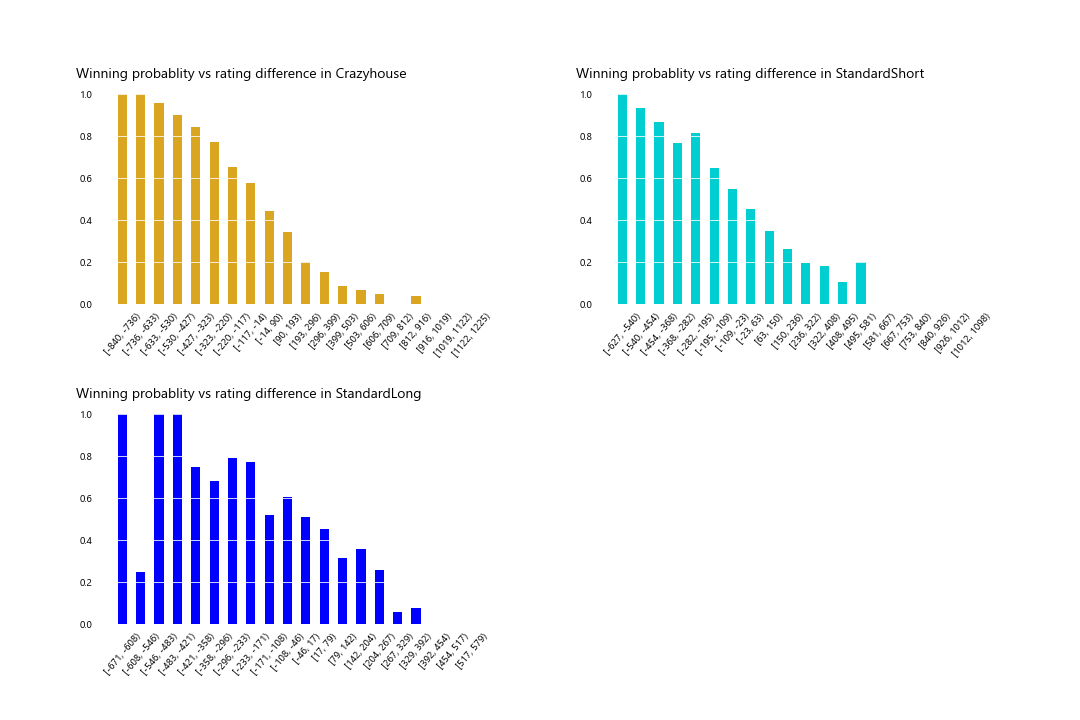
\includegraphics[width=\textwidth]{../img/winning_probabilities_vs_rating.png}
    \caption{Histogram showing winning probabilities when rating difference between I and opponent.}
    \label{fig:winning probabilities}
\end{figure}

% Bivariate analysis (analysis of bivariate dependencies, visualization) --- max 1 p.
\section{Bivariate Correspondence Analysis}
\label{sec:bivariate}

Chess game can end in three different ways. Player can win, lose or game can be a draw. In this section I study using attraction repulsion matrix and bivariate correspondence analysis how color of chess pieces, chess variant and time of the day affect the game result. I have selected only those standard and crazyhouse chess games in which my opponent have been at least 100 rating points stronger than me.

In figure \ref{fig:color vs result} a heat map presentation of an attraction repulsion matrix between color of chess pieces and game result is shown. I can see that when playing with white pieces I win more often than when playing with black pieces. I also see that interestingly having black pieces makes slightly more probable for the game to end in a draw.

\begin{figure}[ht!]
    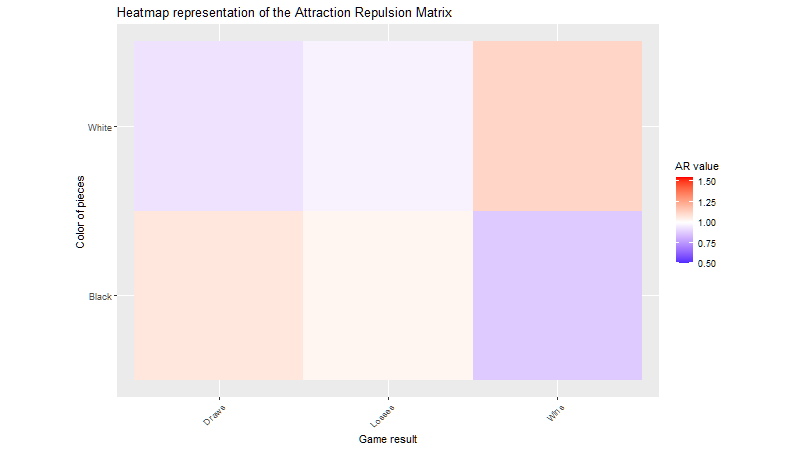
\includegraphics[width=\textwidth]{../img/color_and_result.png}
    \caption{Heat map presentation of attraction repulsion matrix between color of chess pieces and game result.}
    \label{fig:color vs result}
\end{figure}

In figure \ref{fig:variant vs result} a visualization of correspondence analysis between chess variant and game result is shown. I see that game ending in a draw is mostly related to classical chess as crazyhouse variant vector points strictly to opposite direction from draw vector. It must be noted that there are much fewer games ending in a draw than games ending in win or loss which makes draw arrow very long in the visual representation. Figure also suggest a weak connection that losing and playing crazyhouse chess are related to each other and winning is related to Standard chess. This is consistent with winning probabilities given in table \ref{tbl:results by variant} but a bit surprising when comparing to figure \ref{fig:winning probabilities} which would suggest that there still exist lot of "probability mass" for winning against strong opponents in crazyhouse chess.

\begin{figure}[ht!]
    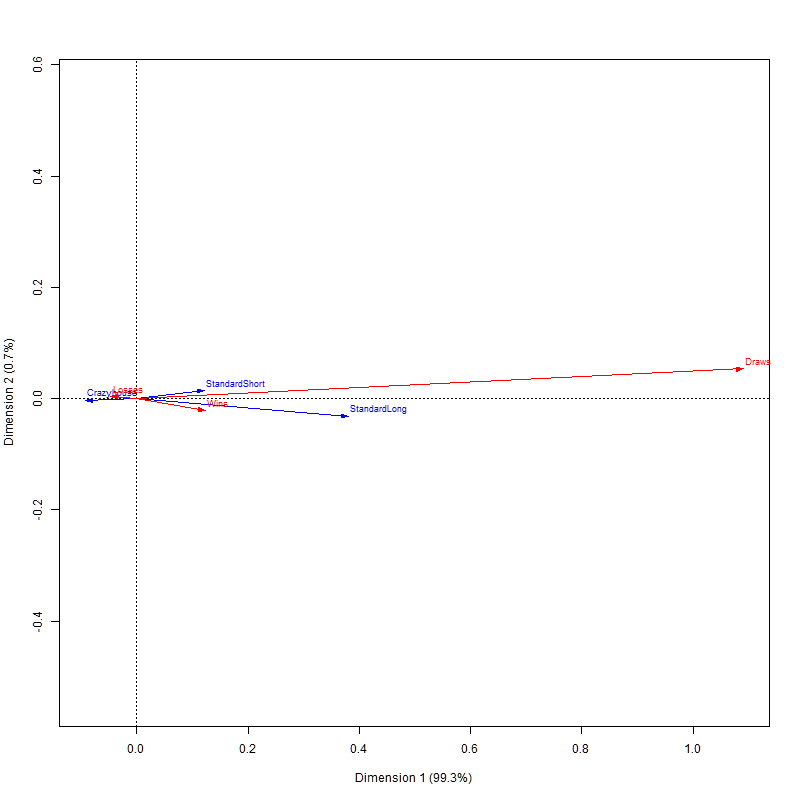
\includegraphics[width=\textwidth]{../img/variant_and_result.png}
    \caption{Visualization of correspondence analysis between chess variant and game result.}
    \label{fig:variant vs result}
\end{figure}

In figure \ref{fig:time vs result} a visualization of correspondence analysis between time of the day and game result is shown. Game has been given label "morning" if it is played before 12 o'clock, label "day" if it is played after 12 o'clock and before 18 o'clock and label "evening" if it has been played after 18 o'clock. This figure shows that in general time of the day and game result doesn't have strong connection despite the small spike in performance at afternoon seen in figure \ref{fig:games vs time of day}. This effect is lost in data aggregation to three categories. Draws and mornings are aligned in the image. I think this is caused by my preference to play longer standard games in morning as standard games tend to end more often in draws than for example in crazyhouse games.

\begin{figure}[ht!]
    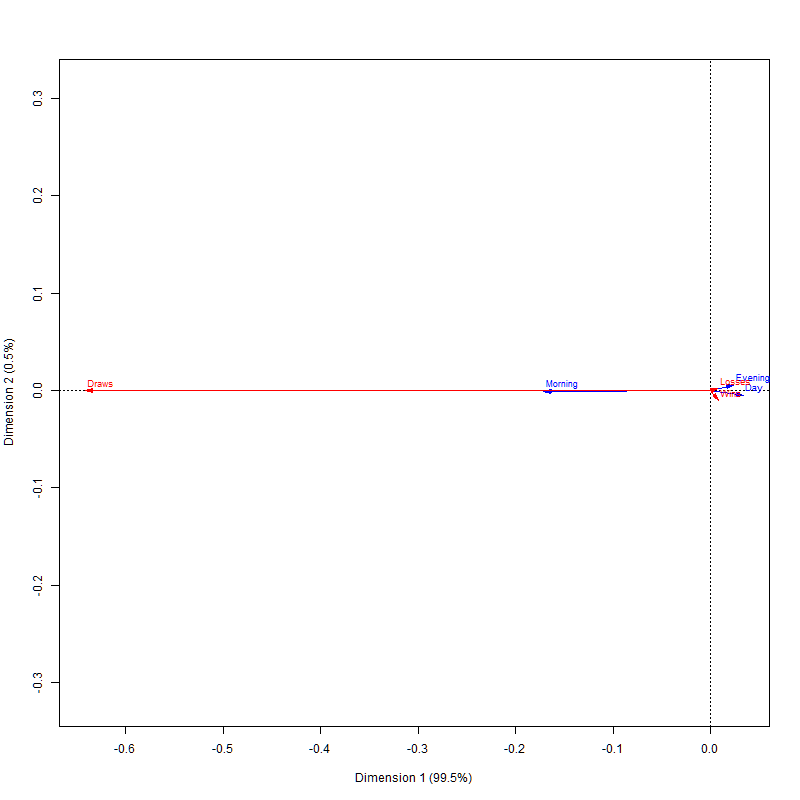
\includegraphics[width=\textwidth]{../img/time_and_result.png}
    \caption{Visualization of correspondence analysis between time of the day and game result.}
    \label{fig:time vs result}
\end{figure}

% Multivariate analysis --- max 3 p. This is divided to selection of the method --- max 1 p.; technical implementation --- max 1 p.; and presenting the results/interpretation --- max 1 p.
\section{Multiple Correspondence Analysis}
\label{sec:multivariate}

In this section I perform multiple correspondence analysis for same variables than were discussed in section \ref{sec:bivariate}. In figure \ref{fig:mca} a visualization of the result of the multiple correspondence analysis between game result, game variant, time of day and color of pieces is shown. I propose following interpretation for the two axes that explain data best. Dimension 1 describes how likely game is to result in a draw. This makes clear distinction between crazyhouse chess and other studied variants because crazyhouse game is very unlike to end in a draw. Dimension 2 can be interpreted as winning-losing axel. Winning is most clearly aligned with having white pieces and somewhat aligned with playing standard chess with long time control. Losing is related to having black pieces and it is somewhat related to playing standard chess with short time control. I don't provide any interpretation for direction related time of day. In this plot connection between losing and crazyhouse chess seen in figure \ref{fig:variant vs result} is not present anymore. This acts as a remainder to be careful when making conclusions from correspondence analysis plots as MCA is non robust method and it is affected a lot by our earlier decision like on how to aggregate data to different categories and how we select threshold for rating difference after which we consider opponent stronger.

\begin{figure}[ht!]
    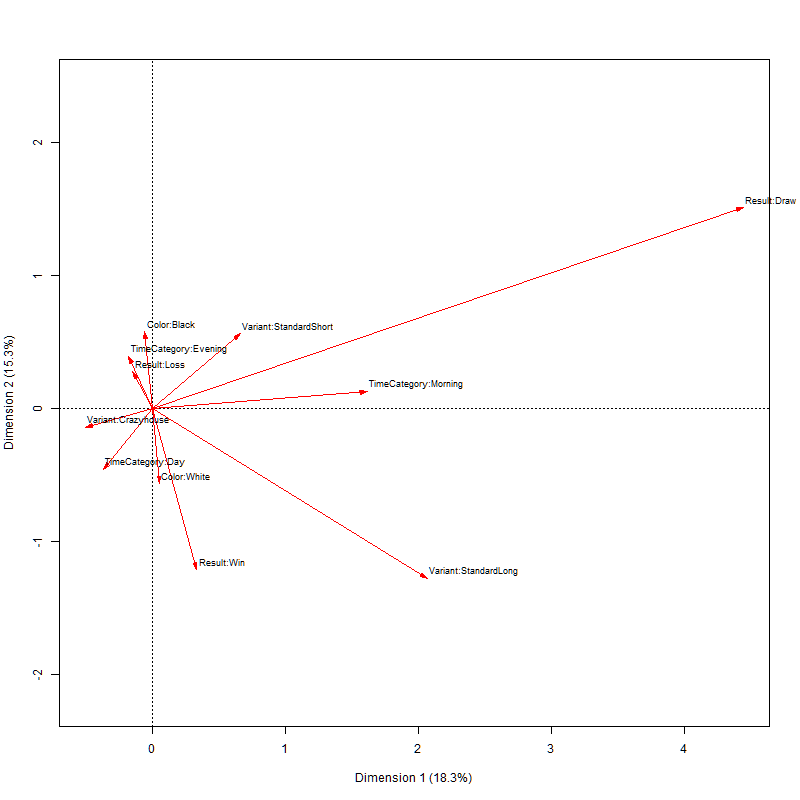
\includegraphics[width=.7\textwidth]{../img/mca.png}
    \caption{Visualization of the result of the multiple correspondence analysis between game result, game variant, time of day and color of pieces.}
    \label{fig:mca}
\end{figure}

% Just because why not
% \input{probability.tex}
% actually just not.

% Critical evaluations (report about possible sources of biases etc.) --- max 0.5 p.
\section{Conclusions}
\label{sec:conclusions}

If I want to maximize my winning changes against stronger opponents I should play with white pieces against them and select standard chess with long time control as our variant. I might also consider timing our game at around 2 PM to benefit from my daily cup of coffee but otherwise timing wasn't shown in our analysis to make a difference.

In addition some less certain observations were made from data. Connection between game ending in a draw and having black pieces can be questioned based on small number of data points since naturally there are a lot less games that end in a draw than games that end in a victory or loss. Also some results suggested connection between higher likelihood of losing and playing crazyhouse variant but other results were against such conclusion. MCA is nonrobust method but we don't see issues with using it in our data as we had good amount of data for performing analysis and our variables had at maximum two or three modalities. Therefore in other respects we are quite confident in our results.

Possible further research could be related on how decisions in data preprocessing affect results. For example time of day could be aggregated to more fine grained categories than just three categories. Similarly changing threshold rating difference on what we consider stronger opponent could lead to new insights. Also similar analysis for other chess variants than discussed here would be interesting but it would also require more data.

% If the report is not polished (blurry images, text in the marginal etc), that may lead to -1p.

\printbibliography
\end{document}